\begin{figure}[hbp]
    \centering
    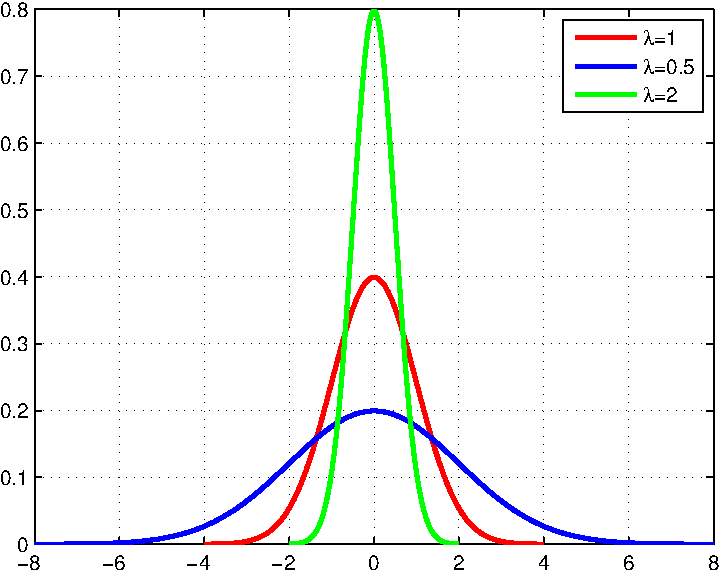
\includegraphics[width=0.6\columnwidth]{Simulation/different_lambda.pdf}
    \caption{$\lambda$ can scale the standard normal distribution to the different range according to the \eqnref{eqn:distribution_scale}.}
    \label{fig:differentlambda}
    \vspace{-2mm}
\end{figure}
\begin{figure*}[!htp]
    \centering
    \subfloat[Raw Data Distribution]{
        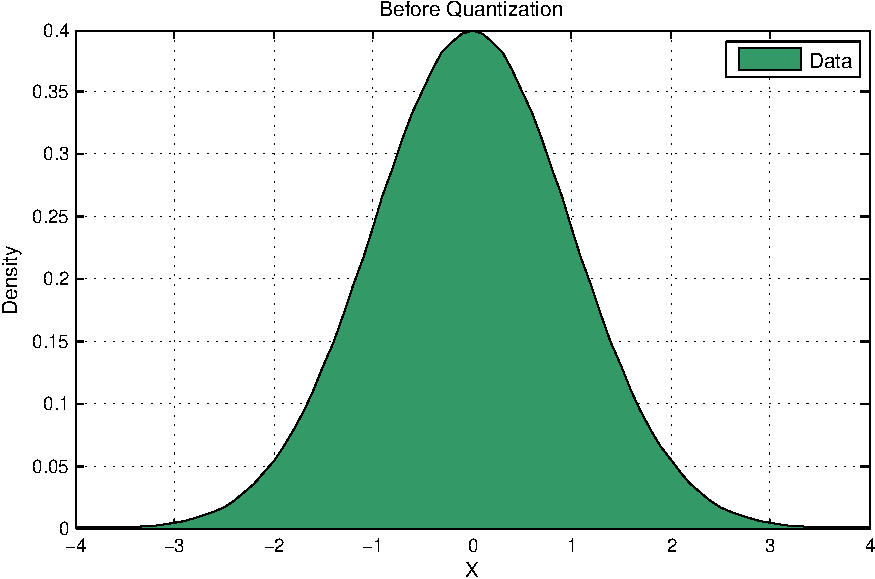
\includegraphics[width=0.33\textwidth]{fig/raw_distribution_croped.pdf}
        \label{fig:before_ulq}
    }~~~~~~~~~~~~~~~~
    \subfloat[Split Data to Regions (R)]{
        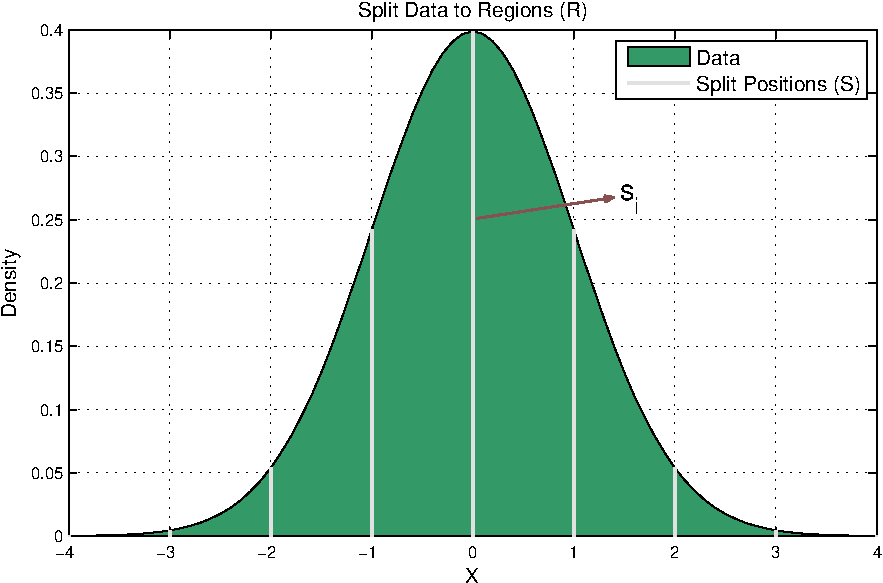
\includegraphics[width=0.33\textwidth]{fig/SplitData2Regions_croped.pdf}
        \label{fig:split_data}
    }\\
    \subfloat[Finding the optimal quantization $q_i\in Q$]{
        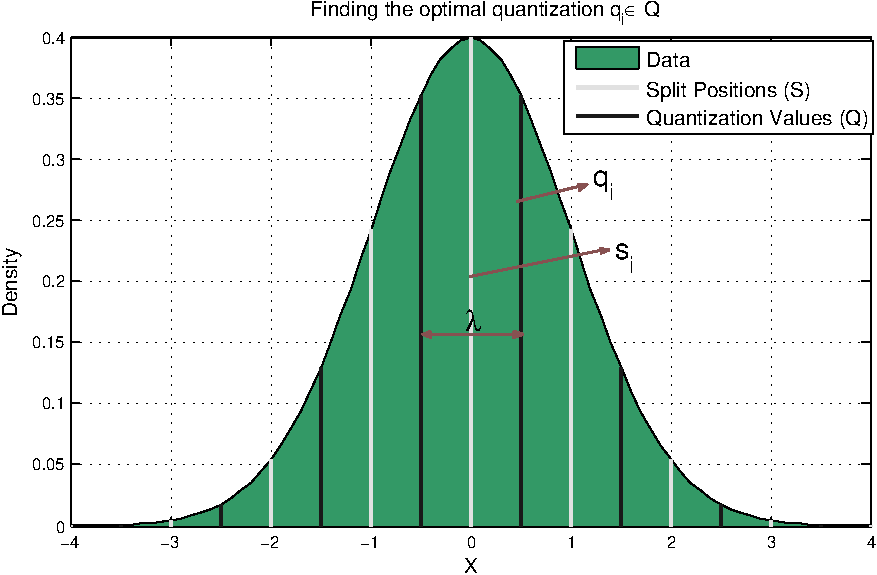
\includegraphics[width=0.33\textwidth]{fig/FindingOptimalQuantization_croped.pdf}
        \label{fig:find_q}
    }~~~~~~~~~~~~~~~~
    \subfloat[Using $q_i$ to represents data in $R_i$]{
        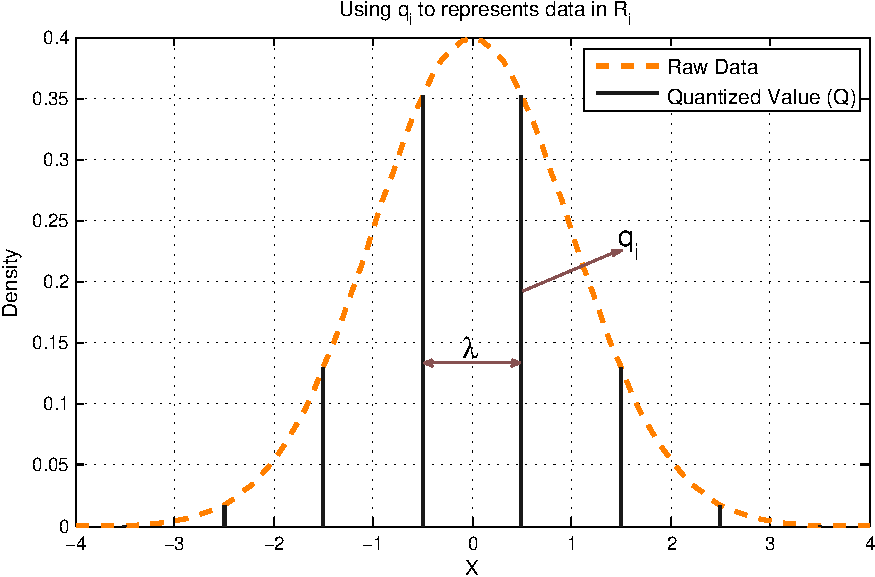
\includegraphics[width=0.33\textwidth]{fig/Q2RepR_croped.pdf}
        \label{fig:after_ulq}
    }
    \caption{The quantization process of $\mu$L2Q. $\varphi$ is the raw data in \figref{fig:before_ulq}, and it be split to $n$ regions $R_i$ by split positions S as shown in \figref{fig:split_data}. The next step is to find the optimal quantization value $q_i\in R_i$ which shown in \figref{fig:find_q}. Finally, all the data in $R_i$ are represented by $q_i$ as shown in \figref{fig:after_ulq}, and our quantization process is done.}
    \label{fig:ulq_process}
\end{figure*}
\section{Optimal Implementation}\label{sec:algo}
%理论到实现需要解决的一些问题
%1、最优位置不等宽
%2、实际中一些位置是没有数据的
%最优量化位置分析:在什么地方量化,损失是最小的
%Based on the discussion above, 
The value of $\lambda$ which is discussed above is the critical factor for low data quantization loss. 
It is used to scale the standard normal distribution to the appropriate range to ensure the lowest data loss after quantization. For example, as shown in \figref{fig:differentlambda}, the data can only be quantized to 4 integers when $\lambda=2$, but if $k>2$, the extra bit width cannot hit the valid data, it caused a waste of bitwidth resource.
When $\lambda=0.5$, data can be quantized to 16 integers, but $k < 4$, the entire data distribution cannot be effectively represented.
So a globally optimal $\lambda$ needs to be analyzed and achieved to solve the issue.

\subsection{Optimality analysis}
To simplify the issue of finding the optimal $\lambda_k$ for $k$-bit width ($k\ge1$), we assume that the quantization is $k$-bit width and let $n = 2^k$.
For the standard normal distribution $\varphi \sim \mathcal{N}(0,1)$, The quantization has three steps:
\begin{itemize}
    \item According to split positions $S=\{s_i|i=1,\cdots,n-1\}$, dividing $\varphi$ into $n$ regions $R_i$.
%\textcolor{blue}{(Cheng: the arrays or sets of value in different range within $\varphi$, that is, $R_i$ is the subset of $\varphi$: $R_i \subset \varphi$.)} 
\begin{equation}
    R_i = \begin{cases}
    \{\varphi_j|\varphi_j>s_{n-1}\};& i=n\\
    \{\varphi_j|s_{i-1}<\varphi_j\le s_{i}\};& i=2, \cdots, n-1\\\
    \{\varphi_j|\varphi_j \le s_1\};&i=1\
    \end{cases}
\end{equation}
%\textcolor{red}{(Cong: what is split position $s_i$? Are they floating point fractional values?)}
Here, $s_i$ is the floating value, and based on $s_i$ the raw data are split to two parts $\{R_i,R_{i+1}\}$ and $R_i \subset \varphi$.
\item  Finding the optimal quantization value $q_i$ in $R_i$; %\textcolor{red}{(Cong: $q_i$ are fixed point values?)}
%\textcolor{blue}{(Cheng: On this section, $q_i$ is floating value, and all the data within $R_i$ will be quantized to $q_i$, that is, all the data in $R_i$ has the same value $q_i$. The optimal meaning is that the loss before and after quantization is minimal.)}
\item Using $q_i$ to represent all values in $R_i$. 
\end{itemize}
Finally, all data in $\varphi$ are quantized into $n$ values, denoted as $Q=\{q_i|i=1,\cdots,n\}$. 
Easy to know, $\lambda=|q_{2}-q_1|=\cdots=|q_{i+1}-q_i|=\cdots=|q_{n}-q_{n-1}|$. Detailed steps are shown in \figref{fig:ulq_process}.%$\lambda$ should be any $|q_{i+1}-q_i|$ but not $|s_{i+1}-s_{i}|$.
%\textcolor{red}{(Cong: what does it mean by "lamda should be any $|q_{i+1}-q_i|$"? Does it mean the value of $\lambda$ equals to any $|q_{i+1}-q_i|$?)}
%\textcolor{blue}{(Cheng: that is $\lambda=|q_{2}-q_1|=\cdots=|q_{i+1}-q_i|=\cdots=|q_{n}-q_{n-1}|$.)}

We define the optimization goal as:
\begin{equation}
    S^*,Q^*=\underset{S,Q}{\arg\min}(J)
\end{equation}
%\textcolor{red}{(Cong: $S*$ and $Q*$ should be defined first or explained here.)}
$S*$ and $Q*$ are the optimal $S$ and $Q$ which make the quantization loss $J$ minimal. $J$ is the loss function defined in \eqnref{eqn:loss_func}.
It could be further expressed with $R_i$ and $q_i$, $J$ as follows:
\begin{align}
\label{eqn:analysis_loss}
        J&=\lVert \varphi-Q \rVert_2^2\nonumber\\
        &=\sum_{i=1}^n(|R_i|q_i^2)-2\sum_{i=1}^n(q_i\sum R_i)+\lVert\varphi\rVert_2^2
\end{align}
Here, $\lVert\varphi\rVert_2^2$ is a constant value that is independent from $Q$ and $S$, and $|R_i|$ denotes the number of elements in $R_i$.
%\textcolor{red}{(Cong: this equation needs to be explained. The $R_i$ are the "regions" defined above; how can a "region" being used in a equation? Does $R_i$ has a value?)}
%\textcolor{blue}{(Cheng: $R_i$ is an array and $R_i \subset \varphi$.)}
We can derive the optimal value of Q as follows:
\begin{align}
    \frac{\partial J}{\partial{q_i}}&=2|R_i|q_i-2\sum{R_i}=0\nonumber\\
    &\Longrightarrow q_i^*=\frac{\sum{R_i}}{|R_i|}=\mu_i
\end{align}

It means, when $q_i^*$ equals to the mean $\mu_i$ of $R_i$, the loss $J$ can be minimized. Based on this, we substitute $q_i^*$ into \eqnref{eqn:analysis_loss} and have:
\begin{equation}
\label{eqn:analysis_C}
    S^*=\underset{S}{\arg\max}(\sum_{1}^{n}(|R_i|u_i^2))
\end{equation}
\eqnref{eqn:analysis_C} has no straightforward solutions. Fortunately, our problem premise is $\varphi\sim \mathcal{N}(0,1)$, so we can approximate this problem by enumerating.
%\textcolor{red}{(Cong: what does "exhausting discrete values"? Do you mean enumerating?)}
%\textcolor{blue}{(Cheng: Yes, it means enumerating.)}

\subsection{Optimal Solution}
Since $\varphi$ in \eqnref{eqn:snd} is known, and it is a standard normal distributed data, we can list all possible situations and find the optimal solution. Our method only finds one parameter $\lambda$, i.e., all $|q_{i+1}-q_{i}|$ should be the same $\lambda$. For $\varphi\sim \mathcal{N}(0,1)$ we need to find the $\lambda_k$ for $k$-bit width quantization that minimizes $J$ in \eqnref{eqn:analysis_loss}. 

\textbf{Data:} Specifically, we generate $N=100000$ data set $\varphi$ that follows the standard normal distribution, and list all possible $\lambda_k$ by a certain interval precision, and select the $\lambda_k$ which minimizes $J$ at $k$-bit width.

\textbf{Range:} Easy to know, $\lambda>0$.
For the upper bound of $\lambda$, given $k$ bits, the range of $\lambda_k$ is $(0, \lambda_{k-1}]$ ($k>1$).
%\textcolor{red}{(Cong: why is $\lambda$'s upper bound is $\lambda_{k-1}$?)}
%\textcolor{blue}{(Cheng: From section III we get that the $\lambda$ is the segmentation width for the standard normal distribution. For every increment of k, double segmentations need to be splited within the standard normal distribution. So  the segmentation width will be reduced, that is, the value of the $\lambda_{k+1}\le\lambda_k$, in order to allow the new segmentations to fall in the valid data area.)}
In addition, we can get that, when $k=1$, the optimal quantization location are the means ($\pm\mu_1,\mu_1>0$) of the two sub-distributions which separated from $\varphi$ by $\varphi$'s mean $\mu$, i.e. $\lambda_1=2\mu_1$.
%\textcolor{red}{(Cong: sorry I did not get this.. sorry for being stupid again but this is not easy to get!..)}
%\textcolor{blue}{(Cheng: The case that $k = 1$ is a special case, in which we only need to split the distribution into two segmentations according to one value. Experiments show that when k=1, it is optimal to split the distribution into two segmentations according to the mean $\mu$ of the data distribution.)}

\textbf{Interval precision:} We take $I=1000$ floating point data within the range of $\lambda_k$, that is $(0, \lambda_{k-1}]$ ($k>1$), to ensure the precision of the approximation. The approximate optimal result is shown in \tabref{tab:optimal_lambda}.

We only give $k = 1$ to $8$ results in \tabref{tab:optimal_lambda}, and more results are not much practical. Because after the bit width is sufficient, the results of evenly quantization is good enough.

\renewcommand{\arraystretch}{1.3}
\begin{table*}[htbp]
\center
    \caption{The list of optimal solution $\lambda$, \textbf{Loss} is the minimum data loss calculating by $J$, and \textbf{Precision} is the interval precision for getting $\lambda$.}
    \label{tab:optimal_lambda}
\begin{tabular}{c|c|c|c|c|c|c|c|c}
\hline
k (bit width)                      & 1      & 2      & 3      & 4      & 5      & 6      & 7      & 8      \\ \hline
$\lambda$ & 1.5959 & 0.9894 & 0.5838 & 0.3327 & 0.1897 & 0.1043 & 0.0563 & 0.0304 \\ \hline
\textbf{Loss}                   & 0.3625 & 0.1189 & 0.0374 & 0.0115 & 0.0035 & 0.0010 & 0.0003 & 0.0001 \\ \hline
\textbf{Precision} & 0.0080 & 0.0050 & 0.0029 & 0.0017 & 0.0009 & 0.0005 & 0.0003 & 0.0002 \\ \hline
\end{tabular}
\end{table*}
%
%解决的思路
\subsection{Algorithm implementation}
%完整的实现算法
Although above analysis was based on a special case of standard normal distribution $\varphi \sim \mathcal{N}(0,1)$, this would make the results look less reliable and may be difficult to apply to the different distributions that actually exist. 
However, it should be noted that, as described in \eqnref{eqn:ulq_method}, our method is based on the premise of normalization of any normal distribution data to the standard normal distribution. 

ULQ can be divided into two steps in Logically: 1) normalize the  $w_f$ which satisfies normal distribution to the standard normal distribution, in this step we record the offset factor $\beta=\mu$ and a part of the scaling factor $\sigma$; 2) Based on the standard normal distribution generated in step 1, we then analyze the optimal parameter $\lambda$ selection and get the complete scaling factor $\alpha=\lambda\sigma$.

The above analysis is reasonable and credible, because the second logical step is based on the standard normal distribution. In terms of implementation, we only use one step to achieve the above two steps. $\mu$L2Q as shown in \algorithmref{alg:ulq}.
\renewcommand{\arraystretch}{1.3}
\begin{algorithm}[htbp] %算法开始 
\caption{Ultra-low loss quantization} %算法的题目 
\label{alg:ulq} %算法的标签 
\begin{algorithmic}[1] %此处的[1]控制一下算法中的每句前面都有标号 
\Require  $w_f \sim \mathcal{N}(\mu,\sigma)$, $k\ge 1$ 
\Ensure $w_q$, $\alpha$, $\beta$ 
% if-then-else 
\If{$k>8$} 
\State $\lambda_k=\frac{max(w_f)-min(w_f)}{2^k-1}$ 
\Else 
\State Get $\lambda_k$ from \tabref{tab:optimal_lambda}
\EndIf 
\State $\alpha = \lambda_k\sigma$ \& $\beta=\mu$ 
\State $\varphi = \frac{w_f-\beta}{\alpha}$
\State $clip_{max}=2^{k-1}$ \& $clip_{min}=1-2^{k-1}$
\State $\varphi= Clip_{(clip_{min},clip_{max})}(\varphi+0.5)$
\State $w_q=Round(\varphi)$
\end{algorithmic} 
\end{algorithm}

\subsection{Integration with DNN training}
For each layer $l$ of forward-propagation, we first quantize $w_f(l)$ to $w_q(l)$. 
And then, $w_q(l)$ is used to calculate the output of each layer $l$ in forward propagation.

During back-propagation, the values in \algorithmref{alg:ulq} are not differentiated, derivatives of $w_q$ are computed instead \citep{zhou2016dorefa,TWNs,gysel2016hardware}, yielding the identity function \eqnref{eqn:gradient}, and $g(l)$ is the gradient of layer $l$.
\begin{equation}
    \label{eqn:gradient}
    g(l)=\frac{\partial J(w_q)}{\partial w_q(l)}=\frac{\partial J(w_q)}{\partial w_f(l)}
\end{equation}

%For a deployment of the NN model on any devices for inference, we only need to save the ternary-valued co-efficients and the scaling values together with the other quantized network parameters if necessary.
